\chapter{Diseño}
\label{ch:diseno}

\section{Sintaxis Abstracta}
\lstsetocl

A continuación se muestra el diagrama de clases \ref{fig:fig2} de
nuestra herramienta:

\todo{AB: porque se nos va la imagen a otra pagina?}
\begin{figure}
  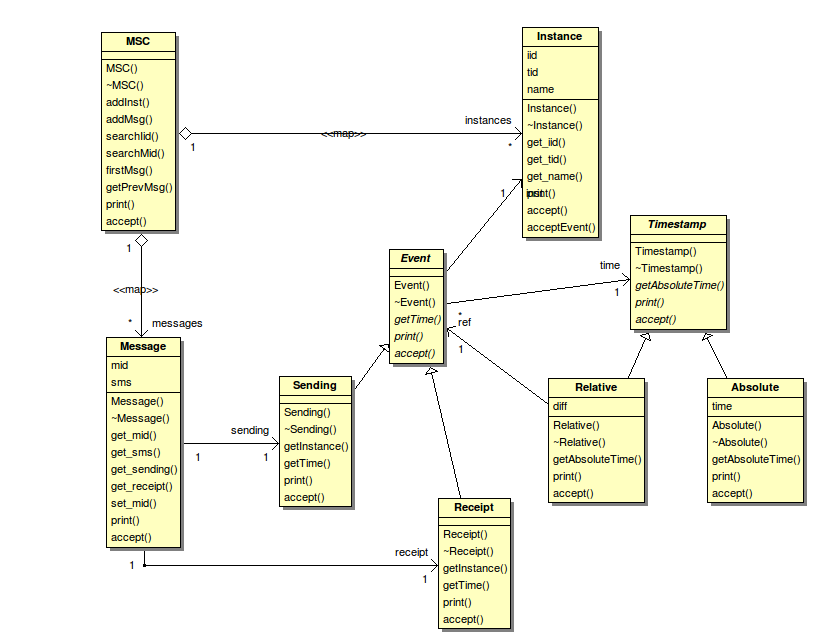
\includegraphics[scale=0.5]{./images/fig2}
  \caption{Ejemplo de una corregion dentro en un msc.}
  \label{fig:fig2}
\end{figure}

A continuación vamos a explicar la representación abstracta respecto a
la concreta:
\begin{itemize}
\item La clase \textit{MSC} representa a nuestro MSC propiamente
  dicho. En él almacenamos las instancias y mensajes que el usuario va
  introduciendo en la comunicación.
\item
\item 
\item 
\item  

\end{itemize}

\section{Arquitectura}

Básicamente la arquitectura de \textit{Progtalk} es la siguiente:
\begin{itemize}
\item En un primer lugar tenemos el analizador léxico. Su labor es ir
  tomando información del fichero de entrada carácter a carácter e ir
  agrupando en \textit{tokens} (unidad mínima de información que
  maneja posteriormente el analizador sintáctico).
\item Los tokens son enviados al analizador sintáctico, el cuál se
  encarga de parsear el fichero de entrada (es decir, va uniendo los
  tokens que va recibiendo y verifica que el fichero entrante esta
  escrito conforme al lenguaje diseñado para describir el universo del
  problema).  Durante el análisis sintáctico del fichero de entrada se
  hace necesario la creación de una serie de objetos los cuales sirven
  como almacenamiento intermedio de la información. La razón para
  hacer esto es la siguiente: imaginemos que estamos parseando una
  línea del fichero de entrada. Lo que el analizador sintáctico (a
  partir de ahora \textit{parser})va a hacer es ir comparando la
  entrada con cada una de las reglas de dicho parser. Se irá creando
  un árbol sintáctico conforme avanza el parseo, y almacenando la
  información leída para que una vez se acepte la línea de entrada
  tengamos toda la información sobre dicha línea recopilada, y podamos
  almacenarla en el objeto\textit{msc} en el cual se almacena toda la
  comunicación antes de generar el fichero \textit{.tex}.

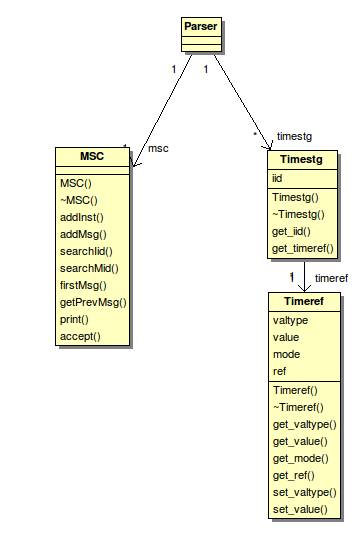
\includegraphics[scale=0.5]{./images/fig3}

\item Para verificar la consistencia de la comunicación tenemos el
  analizador semántico. En este punto, debemos explicar que parte de
  este análisis se ha realizado durante el análisis sintáctico, y
  parte se ha realizado tras la finalización de éste. La razón por la
  que tomamos esta decisión es que algunas verificaciones de
  consistencia, como por ejemplo la no duplicidad de identificadores,
  era fácil de empotrar dentro del código del analizador sintáctico,
  optimizando el funcionamiento de \textit{Progtalk} sin aumentar la
  complejidad del código, mientras que otras verificaciones como por
  ejemplo la consistencia de los tiempos de envío y recepción, eran
  suficientemente complejas como para diferir su procesado,
  simplificando así mucho el código.
\item Por ultimo tenemos el generador de código, que lee toda la
  comunicación procesada y almacenada en memoria, y la exporta al
  formato requerido por el usuario.
\end{itemize}

\section{Análisis Léxico}
Para implementar el analizador léxico (al cual hemos llamado
\textit{Scanner}) hemos usado flex++. Los tokens que hemos definido
para el universo de nuestro problema son:

\begin{itemize}
\item NUM: cualquier número entero.
\item ID: cualquier identificador comenzado en letra y formado por
  letras, números o el símbolo ''\_''.
\item WHITE: cualquier espacio en blanco o tabulador.
\item STRING: cualquier conjunto de caracteres entre comillado salvo
  comillas o salto de línea.
\item EOLN: uno o más saltos de línea.
\item INSTANCE: el literal ''instance".
\item OF: el literal "of".
\item MESSAGE: el literal "message".
\item FROM: el literal ''from''.
\item TO: el literal ''to''.
\item AT: el literal ''@''.
\item PLUS: el literal ''+''.
\item MINUS: el literal ''-''.
\item EXCLAMATION: el literal ''!''.
\item INTERROGATION: el literal ''?''.
\item SEMICOLON: el literal '';''.
\item LEFT\_BRACE: el literal ''\{''.
\item RIGHT\_BRACE: el literal ''\}''.
\end{itemize}

\section{Análisis Sintáctico}

Para implementar el analizador sintáctico (al cual hemos llamado
\textit{Parser}) hemos usado \textit{bisonc++}. El proceso de parseo
es el siguiente. El objeto \textit{Parser} va tomando los tokens
enviados por \textit{Scanner} y comprueba que el lenguaje que esta
leyendo es un lenguaje correcto. En caso de no serlo se aborta el
proceso de parseo y el programa termina.

Las acciones semánticas en \emph{bisonc++} simplemente construyen los
nodos del árbol de sintaxis abstracta. Veamos un ejemplo de una de
nuestras acciones semánticas: \lstsetc
\begin{lstlisting}
message:
     MESSAGE mid_opt string_opt origin_opt destiny_opt SEMICOLON EOLN
        { 
	      string * mid = $2;
          string * desc = $3;
          Timestg * orig = $4;
          Timestg * dest = $5;
        }
	  if (mid == NULL)
	    mid = new string("No_Info_Available");

	  if (desc == NULL)
	    desc = new string("");

	  if (orig == NULL)
	    {
	      std::cout << "ERROR: User didn't provide message's origin" 
			<< std::endl;
	      exit(-1);
	    }

	  if (dest == NULL)
	    {
	      std::cout << "ERROR: User didn't provide message's destiny" 

			<< std::endl;
	      exit(-1);
	    }
	     addMsg(*mid, *desc, orig->get_iid(), dest->get_iid(), 
		 orig->get_timeref(), dest->get_timeref());
	}
;
\end{lstlisting}

Se puede observar cómo el símbolo no terminal \lstinline{message} bla bla bla

\section{Análisis Semántico}

En nuestro programa parte del análisis semántico se realiza de forma
paralela al análisis sintáctico y parte se realiza tras finalizar
éste. En concreto, las inconsistencias que se reconocen durante el
análisis sintáctico son:
\begin{itemize}
\item La declaración de varias instancias con igual identificador,
\item la declaración de varios mensajes con igual identificador,
\item la ausencia de elementos imprescindibles de un mensaje, como su
  origen o destino,
\item la referencia a un mensaje o instancia que no ha sido declarado
  anteriormente.
\end{itemize}

El hecho de detectar estas inconsistencias nada más producirse, nos da
la ventaja de evitar el procesado de una comunicación errónea,
ahorrando tiempo y recursos.

Una vez terminado este proceso con éxito, pasamos a la segunda parte
del análisis semántico donde comprobaremos la consistencia en los
tiempos de envío y recepción de los mensajes. Hay dos razones por las
que nos hemos realizado esta comprobación en paralelo con el análisis
sintáctico:
\begin{itemize}
\item Por un lado, durante la fase de análisis del problema, tomamos
  la decisión de intentar almacenar la información del fichero de
  entrada tan fielmente como fuera posible para así poder dar marcha
  atrás si lo deseáramos y obtener de nuevo el fichero de entrada a
  partir del la información parseada y almacenada. Esto implica que
  los tiempos relativos se almacenan como referencias y no como
  valores absolutos, lo que hace imposible comprobar su integridad
  hasta el final del parseo,
\item y por otro lado, comprendimos que el código del analizador
  sintáctico se volvería demasiado complejo y poco legible si
  finalmente incluíamos este tipo de verificaciones durante esta fase.
\end{itemize}

Para la implementación de esta parte del analizador semántico hemos
usado un patrón \textit{Visitor}~\cite{gof}.

\section{Generación de Código}

Para esta tarea hemos utilizado un patrón de diseño \textit{Visitor},
el cual recorre toda la información almacenada y a partir de ésta crea
un fichero \textit{.tex} que compilado en \textit{latex} nos dará una
representación gráfica de la comunicación.


%%% Local Variables: 
%%% mode: latex
%%% TeX-master: "progtalk"
%%% TeX-PDF-mode: t
%%% ispell-local-dictionary: "castellano"
%%% End: 
